\begin{figure}[H]
    \centering
    \begin{tikzpicture}[
        node distance=1cm and 3mm,
        every node/.style={
            draw,
            align=center,
            font=\scriptsize,
            text width=1.6cm,
            minimum height=0.7cm
        },
        lymphprecursor/.style={fill=Purple!20},
        lymphmature/.style={fill=Purple!60},
        lymphmature2/.style={fill=Purple},
        myeloprecursor/.style={fill=Rhodamine!30},
        myelomature/.style={fill=Rhodamine!70},
        img/.style={draw=none, minimum height=0mm, inner sep=0pt}
    ]

    % Root node
    \node (csh) [text width=4cm] {Cellule souche  hématopoïétique multipotente (CSH)};

    % Myeloid branch
    \node (myeloid) [below left=of csh, myeloprecursor] {Progéniteur  myéloïde};

    \node (erytho) [below=of myeloid, myeloprecursor] {Érythroblaste};
    \node (megaka) [left=of erytho, myeloprecursor] {Mégacaryocyte};
    \node (monoblast) [right=of erytho, myeloprecursor] {Monoblaste};
    \node (myeloblast) [right=of monoblast, myeloprecursor] {Myéloblaste};

    \node (plaq) [below=of megaka, myelomature] {Plaquette};
    \node (gr)   [below=of erytho, myelomature] {Globule  rouge};

    \node (mono)  [below=of monoblast, myelomature] {Monocyte};
    \node (eosino) [below=3.5cm of myeloblast, myelomature] {Granulocyte  éosinophile};
    \node (neutro) [right=of eosino, myelomature] {Granulocyte  neutrophile};
    \node (baso)   [right=of neutro, myelomature] {Granulocyte  basophile};


    % Lymphoid branch
    \node (lymphoid) [right=8cm of myeloid, lymphprecursor] {Progéniteur  lymphoïde};

    \node (bcell) [below=of lymphoid, lymphmature] {Lymphocyte B};
    \node (tcell) [right=of bcell, lymphmature] {Lymphocyte T};
    \node (nkcell) [left=of bcell, lymphmature] {Cellule NK};
    \node (plasmocyte) [below=of bcell, lymphmature2] {Plasmocyte};

    % Images
    \node[img, below=2pt of plaq] {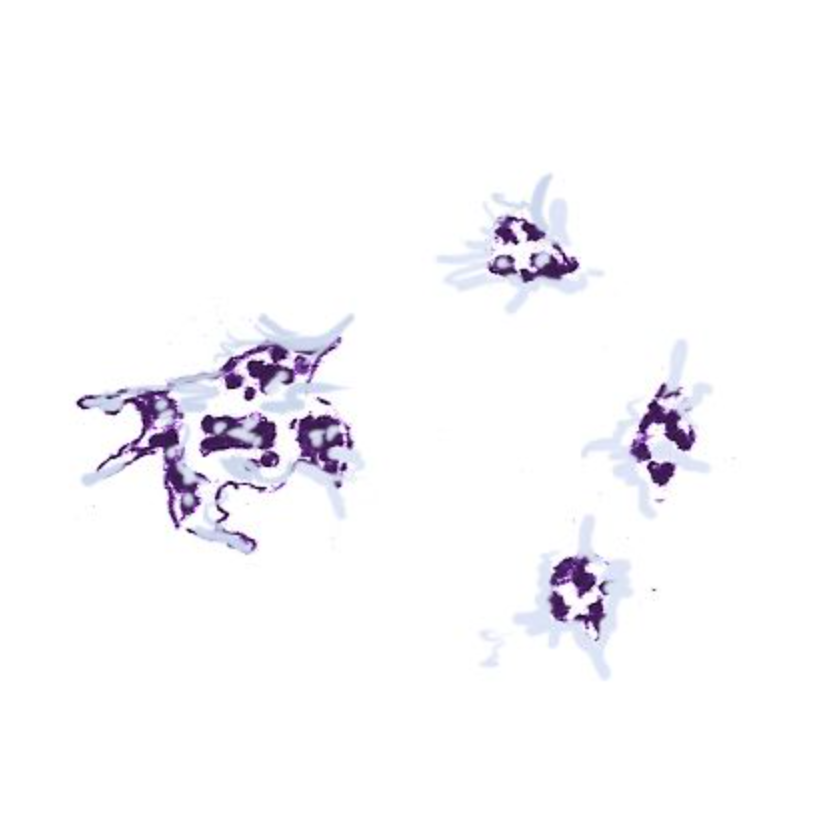
\includegraphics[width=1.5cm]{images/plt.png}};
    \node[img, below=2pt of gr] {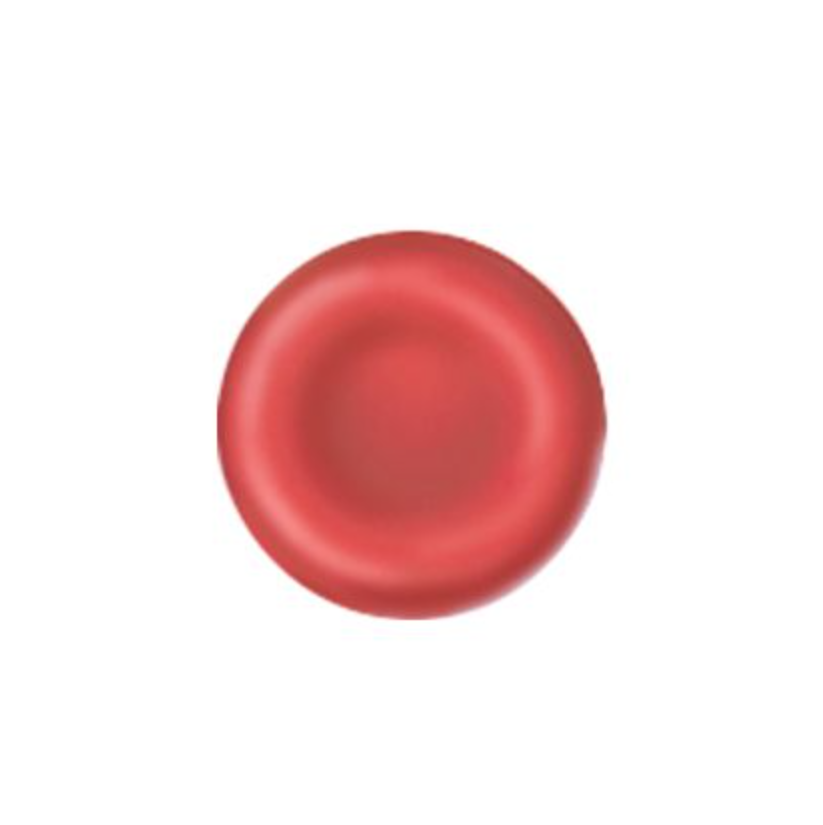
\includegraphics[width=1.5cm]{images/gr.png}};
    \node[img, below=2pt of mono] {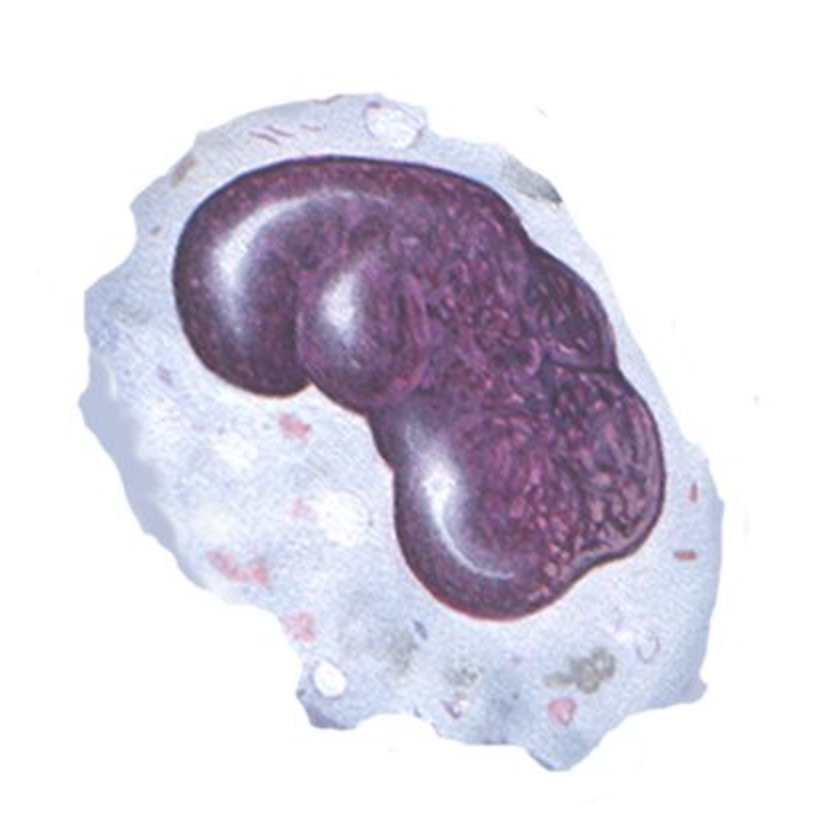
\includegraphics[width=1.5cm]{images/monocyte.png}};
    \node[img, below=2pt of eosino] {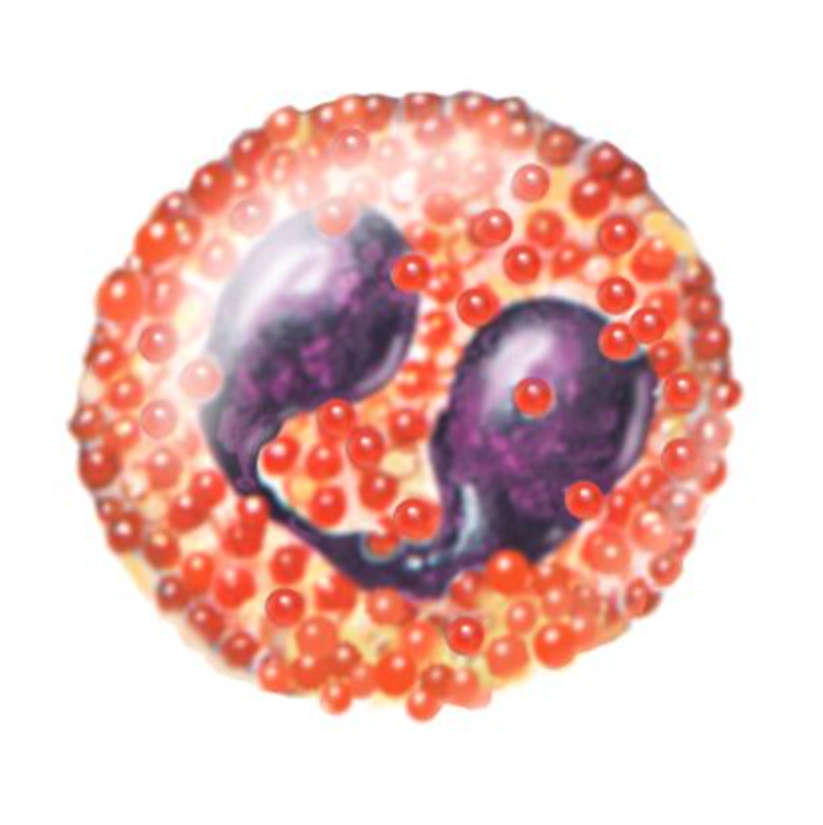
\includegraphics[width=1.5cm]{images/pne.png}};
    \node[img, below=2pt of neutro] {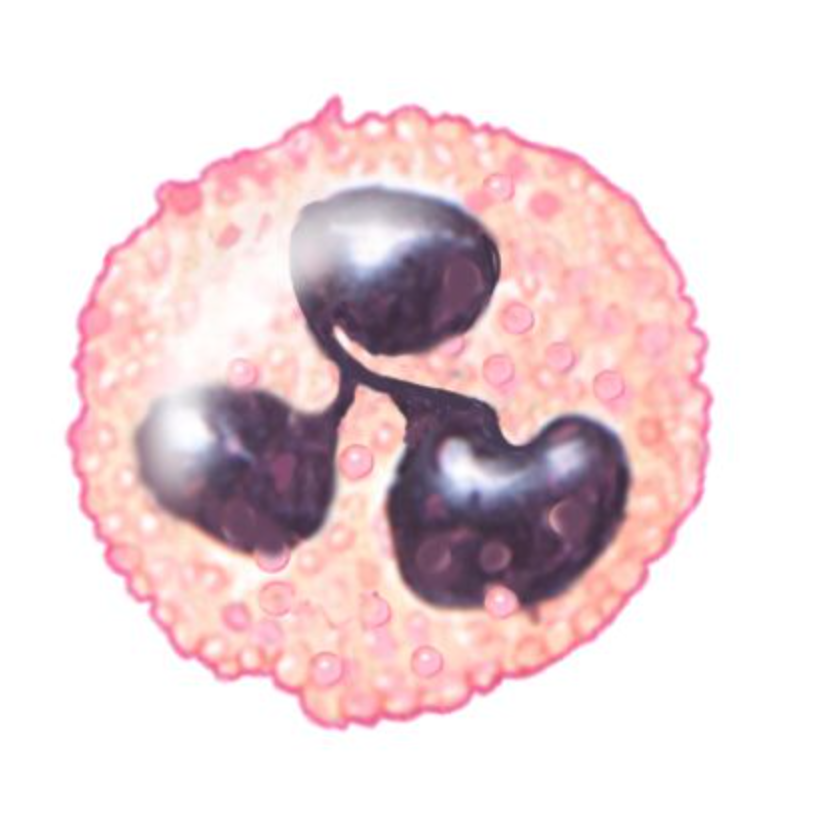
\includegraphics[width=1.5cm]{images/pnn.png}};
    \node[img, below=2pt of baso] {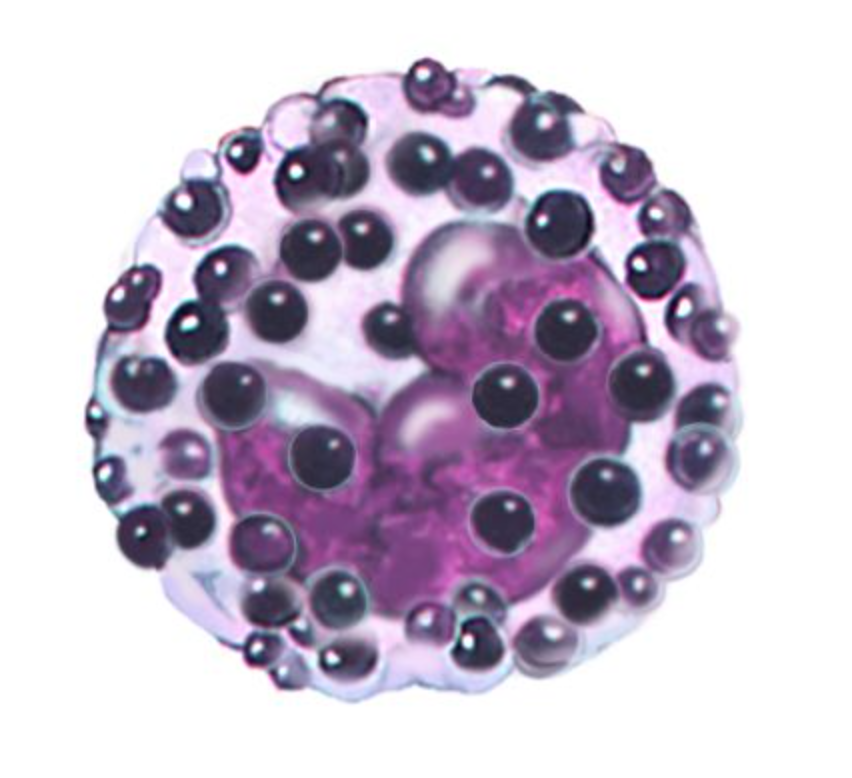
\includegraphics[width=1.5cm]{images/pnb.png}};
    \node[img, below right=1.5pt of bcell] {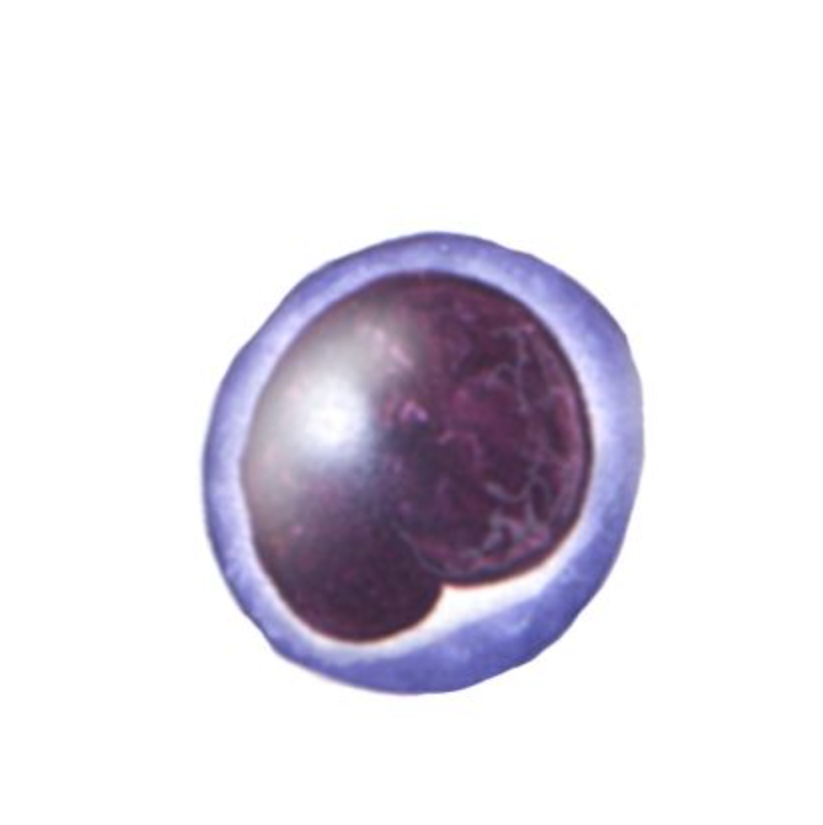
\includegraphics[width=1.5cm]{images/lympho.png}};
    \node[img, below=2pt of plasmocyte] {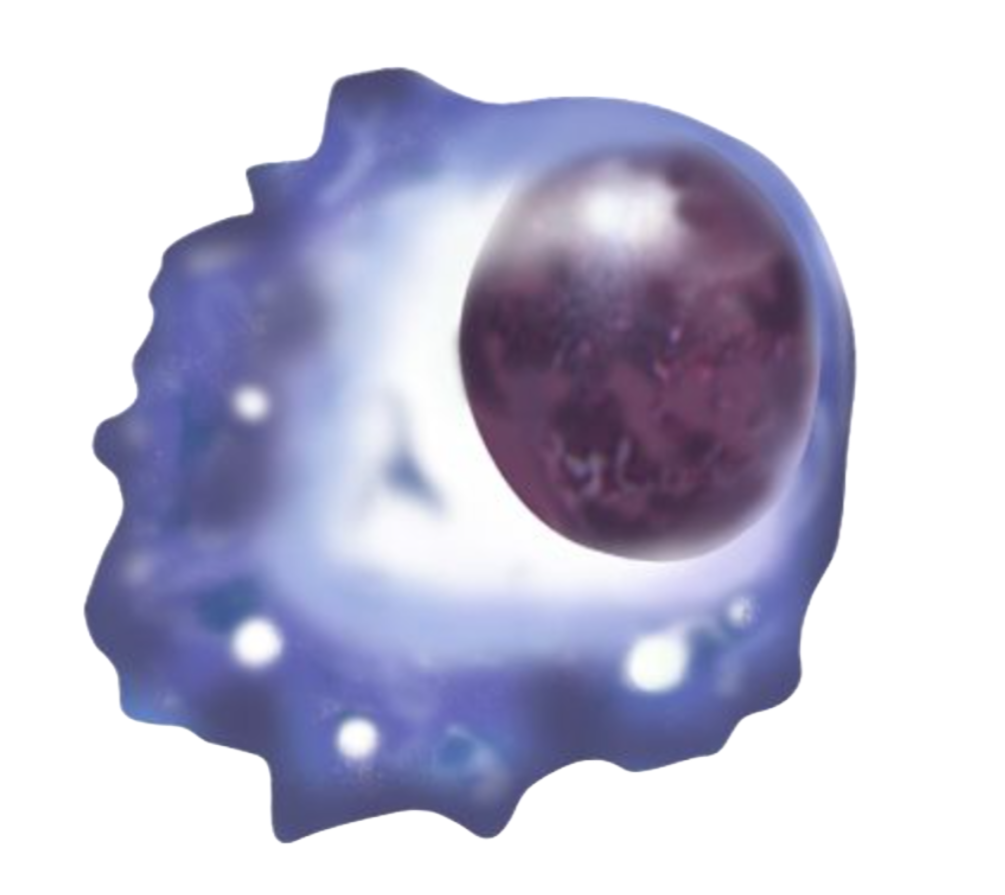
\includegraphics[width=1.5cm]{images/plasmo.png}};
    \node[img, below=5pt of nkcell] {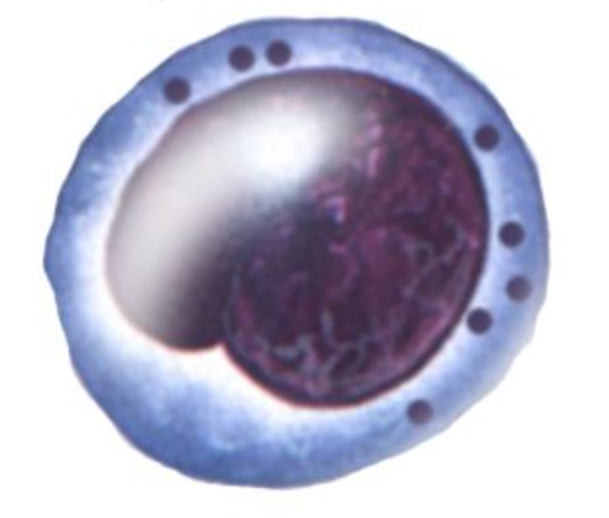
\includegraphics[width=1.5cm]{images/lynk.png}};

    % Disease boxes
    \node[
        fit=(myeloid)(erytho)(monoblast)(myeloblast), 
        draw=Rhodamine!40, 
        dotted, 
        ultra thick, 
        inner sep=5pt, 
        label=above right:{\textbf{\textcolor{Rhodamine!40}{LAM}}}
    ] {};

    \node[
        fit=(baso)(eosino)(neutro), 
        draw=Rhodamine, 
        dotted, 
        ultra thick, 
        inner sep=5pt, 
        label=above left:{\textbf{\textcolor{Rhodamine}{LMC}}}
    ] {};

    \node[
        fit=(plaq)(gr)(mono), 
        draw=Rhodamine, 
        dotted, 
        ultra thick, 
        inner sep=5pt, 
        label=above right:{\textbf{\textcolor{Rhodamine}{SMP}}}
    ] {};

    \draw[
    draw=Purple!40, 
    dotted, 
    ultra thick, 
    ]
    ($(lymphoid.south west) + (-3pt,-3pt)$)
    rectangle
    ($(lymphoid.north east) + (3pt,3pt)$);

    \node[draw=none, thick, text=Purple!40] 
    at ($(lymphoid.north) + (0,0.5cm)$) 
    {\textbf{LAL}};

    \node[
        fit=(nkcell)(bcell)(tcell), 
        draw=Purple!60, 
        dotted, 
        ultra thick, 
        inner sep=5pt, 
        label={[xshift=-15pt]above left:{\textbf{\textcolor{Purple!60}{SLP/LNH}}}}
    ] {};

    \draw[
        draw=Purple!60, 
        dotted, 
        ultra thick, 
        ]
        ($(bcell.south west) + (-3pt,-10pt)$)
        rectangle
        ($(bcell.north east) + (3pt,10pt)$);
    
    \node[draw=none, thick, text=Purple!60] 
    at ($(bcell.north) + (0.5,0.6cm)$) 
    {\textbf{LLC}};

    \draw[
        draw=Purple,
        line width=3pt,
        line cap=rect,
        dash pattern=on 0pt off 6pt,
    ]
        ($(plasmocyte.south west) + (-3pt,-3pt)$)
        rectangle
        ($(plasmocyte.north east) + (3pt,3pt)$);    

    \node[draw=none, thick, text=Purple] 
    at ($(plasmocyte.west) + (-0.5,0cm)$) 
    {\textbf{MM}};

    % Connections
    \draw[-] (csh) -- (myeloid);
    \draw[-] (csh) -- (lymphoid);

    \draw[-] (myeloid) -- (erytho);
    \draw[-] (myeloid) -- (megaka);
    \draw[-] (myeloid) -- (myeloblast);
    \draw[-] (myeloid) -- (monoblast);

    \draw[-] (megaka) -- (plaq);
    \draw[-] (erytho) -- (gr);
    \draw[-] (myeloblast) -- (neutro);
    \draw[-] (myeloblast) -- (eosino);
    \draw[-] (myeloblast) -- (baso);
    \draw[-] (monoblast) -- (mono);

    \draw[-] (lymphoid) -- (bcell);
    \draw[-] (lymphoid) -- (tcell);
    \draw[-] (lymphoid) -- (nkcell);
    \draw[-] (bcell) -- (plasmocyte);

    \end{tikzpicture}
    \caption{
        Classification des hémopathies malignes selon la lignée cellulaire d'origine 
        (\colorbox{Rhodamine!60}{myéloïde} à gauche ou \colorbox{Purple!60}{lymphoïde} à droite) 
        et le stade de maturation des cellules (\colorbox{Gray!20}{immature} en haut et \colorbox{Gray!70}{mature} en bas).
        LAM : leucémies aiguës myéloïdes, LAL : leucémies aiguës lymphoblastiques, SMP : syndromes myéloprolifératifs, 
        LMC : leucémie myéloïde chronique, SLP : syndromes lymphoprolifératifs, LNH : lymphomes non hodgkiniens, 
        LLC : leucémie lymphoïde chronique, MM : myélome multiple.
    }
    \label{fig:hemopathies}
\end{figure}
